\appendix

% \section{Alternative prototypes for QS}
% \label{sec:appendix_interface_alternative}


\section{List of Options}
We provide the full list of options presented on the survey.

\begin{itemize}
    \item \textbf{Animal Rights, Welfare, and Services:} Protect animals from cruelty, exploitation and other abuses, provide veterinary services and train guide dogs.
    \item \textbf{Wildlife Conservation:} Protect wildlife habitats, including fish, wildlife, and bird refuges and sanctuaries.
    \item \textbf{Zoos and Aquariums:} Support and invest in zoos, aquariums and zoological societies in communities throughout the country.
    \item \textbf{Libraries, Historical Societies and Landmark Preservation:} Support and invest public and specialized libraries, historical societies, historical preservation programs, and historical estates.
    \item \textbf{Museums:} Support and invest in maintaining collections and provide training to practitioners in traditional arts, science, technology, and natural history.
    \item \textbf{Performing Arts:} Support symphonies, orchestras, and other musical groups; ballets and operas; theater groups; arts festivals; and performance halls and cultural centers.
    \item \textbf{Public Broadcasting and Media:} Support public television and radio stations and networks, as well as providing other independent media and communications services to the public.
    \item \textbf{Community Foundations:} Promote giving by managing long-term donor-advised charitable funds for individual givers and distributing those funds to community-based charities over time.
    \item \textbf{Housing and Neighborhood Development:} Lead and finance development projects that invest in and improve communities by providing utility assistance, small business support programs, and other revitalization projects.
    \item \textbf{Jewish Federations:} Focus on a specific geographic region and primarily support Jewish-oriented programs, organizations and activities through grantmaking efforts
    \item \textbf{United Ways:} Identify and resolve community issues through partnerships with schools, government agencies, businesses, and others, with a focus on education, income and health.
    \item \textbf{Adult Education Programs and Services:} Provide opportunities for adults to expand their knowledge in a particular field or discipline, learn English as a second language, or complete their high school education.
    \item \textbf{Early Childhood Programs and Services:} Provide foundation-level learning and literacy for children prior to entering the formal school setting.
    \item \textbf{Education Policy and Reform:} Promote and provide research, policy, and reform of the management of educational institutions, educational systems, and education policy.
    \item \textbf{Scholarship and Financial Support:} Support and enable students to obtain the financial assistance they require to meet their educational and living expenses while in school.
    \item \textbf{Special Education:} Provide services, including placement, programming, instruction, and support for gifted children and youth or those with disabilities requiring modified curricula, teaching methods, or materials.
    \item \textbf{Youth Education Programs and Services:} Provide programming, classroom instruction, and support for school-aged students in various disciplines such as art education, STEM, outward bound learning experiences, and other programs that enhance formal education.
    \item \textbf{Botanical Gardens, Parks, and Nature Centers:} Promote preservation and appreciation of the environment, as well as leading anti-litter, tree planting and other environmental beautification campaigns.
    \item \textbf{Environmental Protection and Conservation:} Develop strategies to combat pollution, promote conservation and sustainable management of land, water, and energy resources, protect land, and improve the efficiency of energy and waste material usage.
    \item \textbf{Diseases, Disorders, and Disciplines:} Seek cures for diseases and disorders or promote specific medical disciplines by providing direct services, advocating for public support and understanding, and supporting targeted medical research.
    \item \textbf{Medical Research:} Devote and invest in efforts on researching causes and cures of disease and developing new treatments.
    \item \textbf{Patient and Family Support:} Support programs and services for family members and patients that are diagnosed with a serious illness, including wish granting programs, camping programs, housing or travel assistance.
    \item \textbf{Treatment and Prevention Services:} Provide direct medical services and educate the public on ways to prevent diseases and reduce health risks.
    \item \textbf{Advocacy and Education:} Support social justice through legal advocacy, social action, and supporting laws and measures that promote reform and protect civil rights, including election reform and tolerance among diverse groups.
    \item \textbf{Development and Relief Services:} Provide medical care and other human services as well as economic, educational, and agricultural development services to people around the world.
    \item \textbf{Humanitarian Relief Supplies:} Specialize in collecting donated medical, food, agriculture, and other supplies and distributing them overseas to those in need.
    \item \textbf{International Peace, Security, and Affairs:} Promote peace and security, cultural and student exchange programs, improve relations between particular countries, provide foreign policy research and advocacy, and United Nations-related organizations.
    \item \textbf{Religious Activities:} Support and promote various faiths.
    \item \textbf{Religious Media and Broadcasting:} Support organizations of all faiths that produce and distribute religious programming, literature, and other communications.
    \item \textbf{Non-Medical Science \& Technology Research:} Support research and services in a variety of scientific disciplines, advancing knowledge and understanding of areas such as energy efficiency, environmental and trade policies, and agricultural sustainability.
    \item \textbf{Social and Public Policy Research:} Support economic and social issues impacting our country today, educate the public, and influence policy regarding healthcare, employment rights, taxation, and other civic ventures.
\end{itemize}

\section{Cognitive Demand Tables}
Here we provide the full qualitative analysis table.

\subsection{Mental Demand Table}
\label{apdx:mental_table}
\begin{table}[h]
   \caption{This table lists all the causes participants mentioned as contributing to their Mental Demand. The shaded cells represent the percentage of participants citing each source of mental demand, allowing for comparison within columns. The abbreviations are: ST (Short Text Interface), SI (Short Two-phase Interface), LT (Long Text Interface), and LI (Long Two-phase Interface). Short and Long refer to the sum across both interfaces; Text and Inter refer to the sum across both survey lengths. We include Sparklines for comparisons across these experiment groups.}
    \label{tbl:mental}
    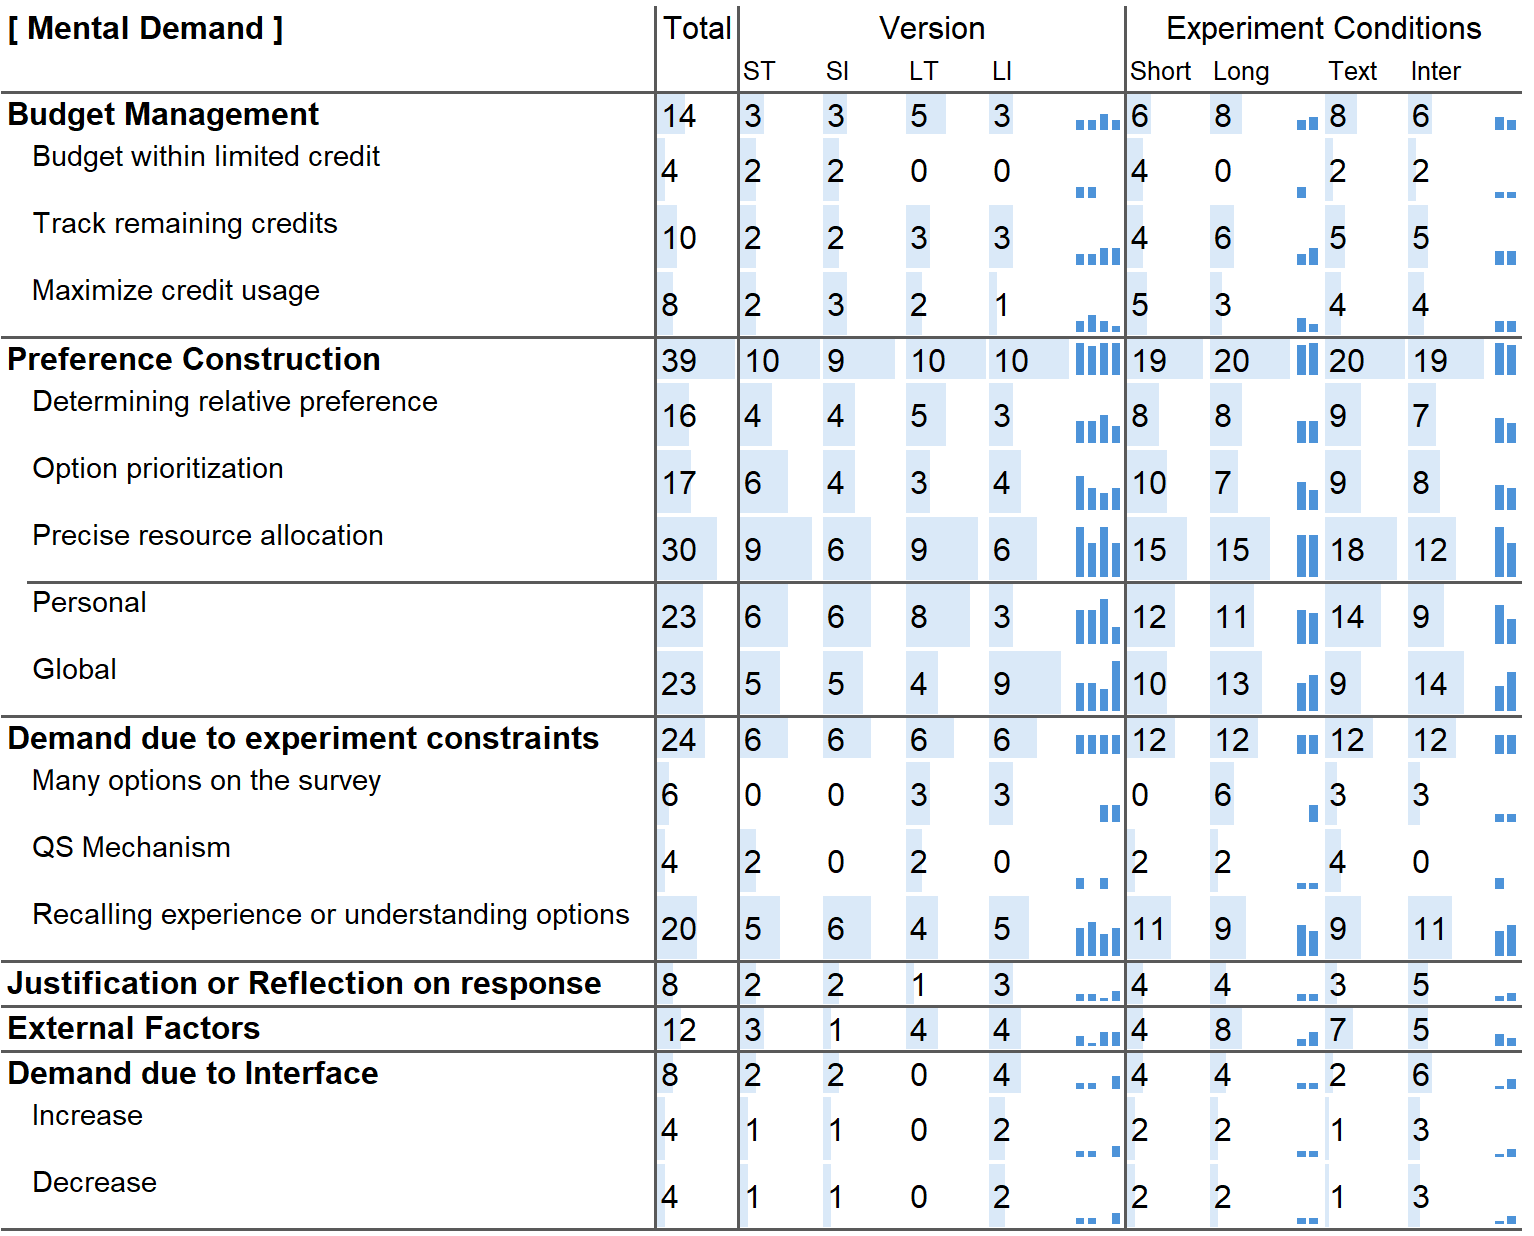
\includegraphics[width=\linewidth]{content/image/cog/mental_table.png}
\end{table}

\subsection{Physical Demand Table}
\label{apdx:physical_table}
\begin{table}[H]
    \caption{Physical Demand Causes: Most participants expressed little or no physical demand. Results reflected that participants in the long two-phase interface required more actions, hence the higher mention of mouse usage as a source.}
    \label{tbl:physical}
    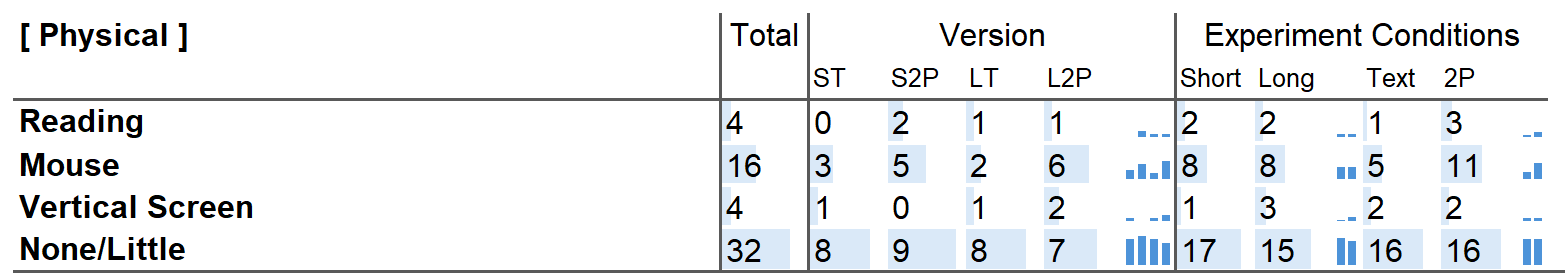
\includegraphics[width=\linewidth]{content/image/cog/physical_table.png}
\end{table}

\subsection{Performance Table}
\label{apdx:perf_table}
\begin{table}[H]
    \caption{Performance Causes: Most causes are shared across experiment conditions. We provided qualitative interpretations of their own perfornace assessments.}
    \label{tbl:physical}
    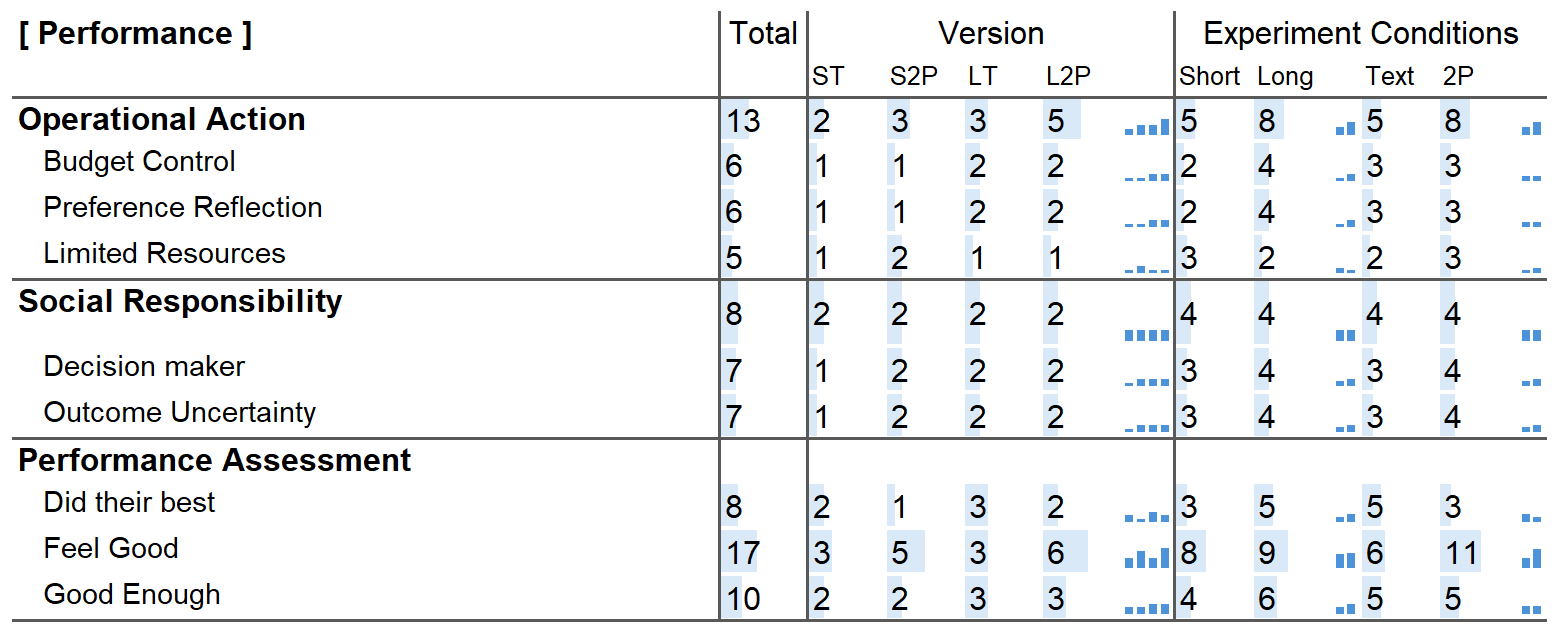
\includegraphics[width=\linewidth]{content/image/cog/perf_table.png}
\end{table}

\subsection{Temporal Demand Table}
\label{apdx:temporal_table}
\begin{table}[H]
    \caption{Temporal Demand Sources: Decision-making and Operational Tasks are the main causes. Participants framed their decision-making sources differently.}
    \label{tbl:temporal}
    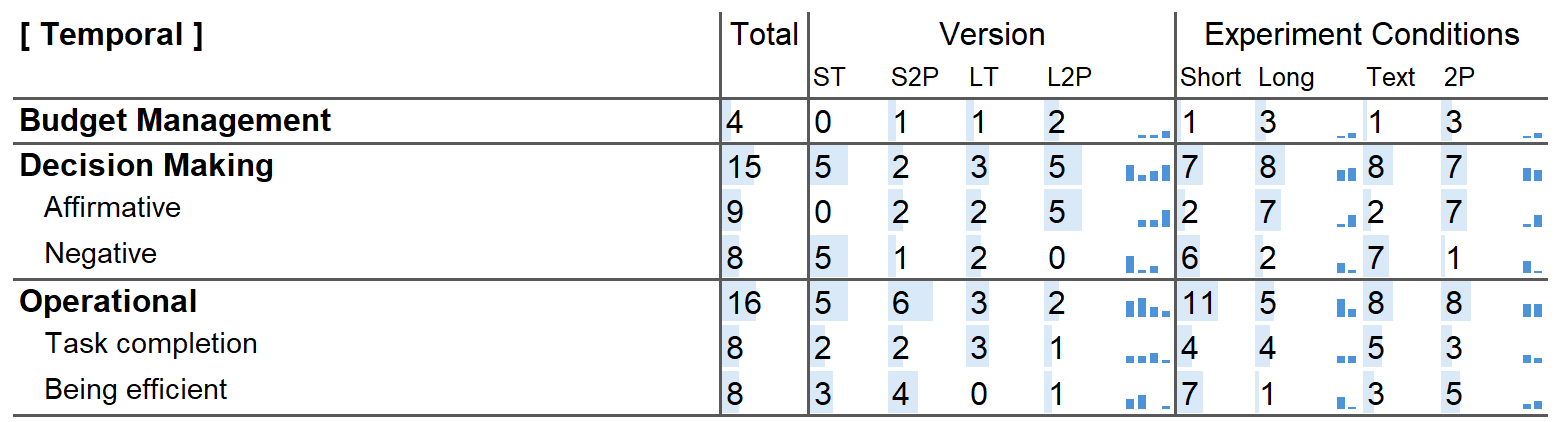
\includegraphics[width=\linewidth]{content/image/cog/temporal_table.png}
\end{table}

\subsection{Frustration Table}
\label{apdx:frus_table}
\begin{table}[H]
    \caption{Frustration Sources: needs to be updated with some new terms definitions for some of the columns.}
    \label{tbl:fustration}
    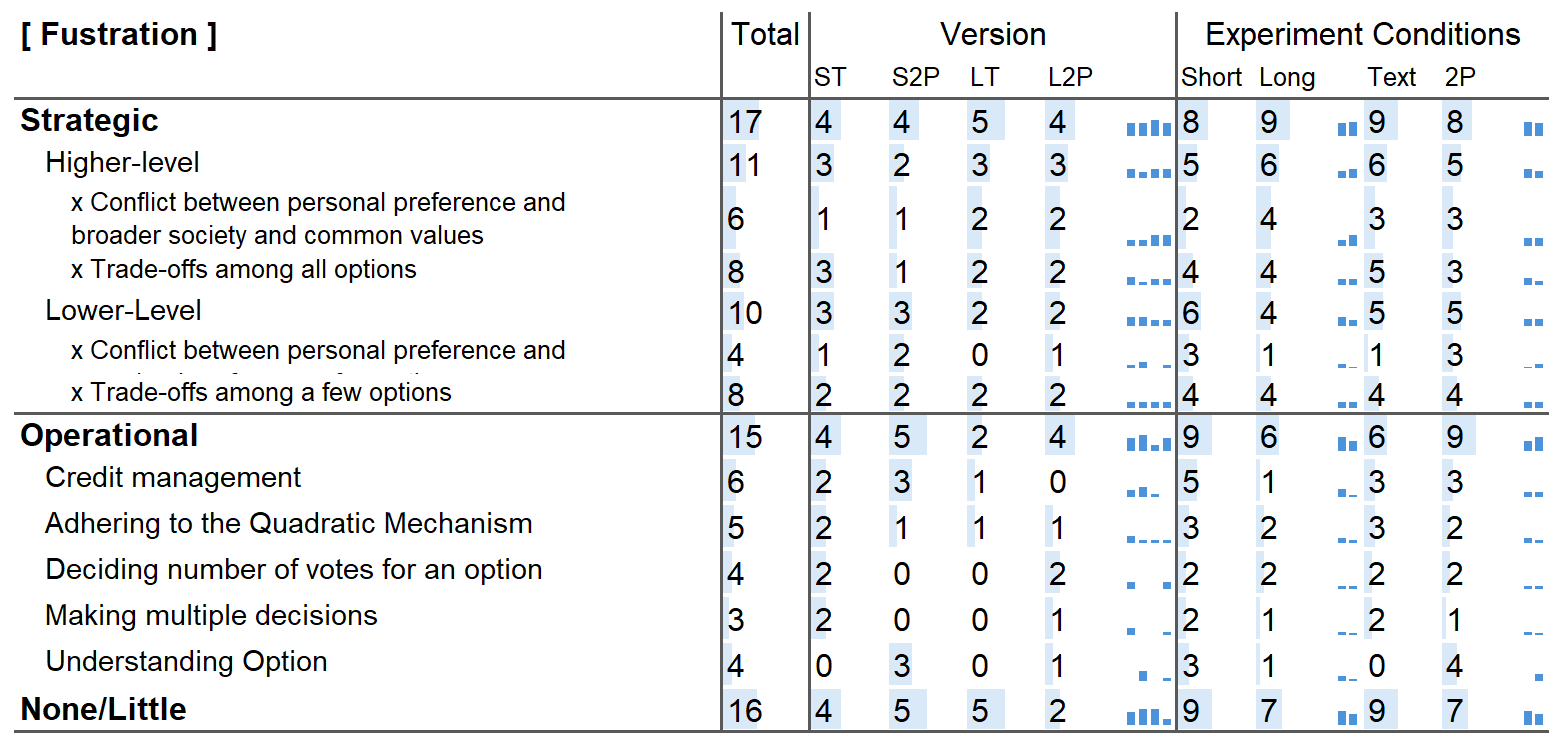
\includegraphics[width=\linewidth]{content/image/cog/fustration_table.png}
\end{table}

